% Options for packages loaded elsewhere
\PassOptionsToPackage{unicode}{hyperref}
\PassOptionsToPackage{hyphens}{url}
\PassOptionsToPackage{dvipsnames,svgnames,x11names}{xcolor}
%
\documentclass[
]{article}

\usepackage{amsmath,amssymb}
\usepackage{iftex}
\ifPDFTeX
  \usepackage[T1]{fontenc}
  \usepackage[utf8]{inputenc}
  \usepackage{textcomp} % provide euro and other symbols
\else % if luatex or xetex
  \usepackage{unicode-math}
  \defaultfontfeatures{Scale=MatchLowercase}
  \defaultfontfeatures[\rmfamily]{Ligatures=TeX,Scale=1}
\fi
\usepackage{lmodern}
\ifPDFTeX\else  
    % xetex/luatex font selection
  \setmainfont[]{Latin Modern Roman}
  \setmathfont[]{Latin Modern Math}
\fi
% Use upquote if available, for straight quotes in verbatim environments
\IfFileExists{upquote.sty}{\usepackage{upquote}}{}
\IfFileExists{microtype.sty}{% use microtype if available
  \usepackage[]{microtype}
  \UseMicrotypeSet[protrusion]{basicmath} % disable protrusion for tt fonts
}{}
\makeatletter
\@ifundefined{KOMAClassName}{% if non-KOMA class
  \IfFileExists{parskip.sty}{%
    \usepackage{parskip}
  }{% else
    \setlength{\parindent}{0pt}
    \setlength{\parskip}{6pt plus 2pt minus 1pt}}
}{% if KOMA class
  \KOMAoptions{parskip=half}}
\makeatother
\usepackage{xcolor}
\setlength{\emergencystretch}{3em} % prevent overfull lines
\setcounter{secnumdepth}{5}
% Make \paragraph and \subparagraph free-standing
\ifx\paragraph\undefined\else
  \let\oldparagraph\paragraph
  \renewcommand{\paragraph}[1]{\oldparagraph{#1}\mbox{}}
\fi
\ifx\subparagraph\undefined\else
  \let\oldsubparagraph\subparagraph
  \renewcommand{\subparagraph}[1]{\oldsubparagraph{#1}\mbox{}}
\fi


\providecommand{\tightlist}{%
  \setlength{\itemsep}{0pt}\setlength{\parskip}{0pt}}\usepackage{longtable,booktabs,array}
\usepackage{calc} % for calculating minipage widths
% Correct order of tables after \paragraph or \subparagraph
\usepackage{etoolbox}
\makeatletter
\patchcmd\longtable{\par}{\if@noskipsec\mbox{}\fi\par}{}{}
\makeatother
% Allow footnotes in longtable head/foot
\IfFileExists{footnotehyper.sty}{\usepackage{footnotehyper}}{\usepackage{footnote}}
\makesavenoteenv{longtable}
\usepackage{graphicx}
\makeatletter
\def\maxwidth{\ifdim\Gin@nat@width>\linewidth\linewidth\else\Gin@nat@width\fi}
\def\maxheight{\ifdim\Gin@nat@height>\textheight\textheight\else\Gin@nat@height\fi}
\makeatother
% Scale images if necessary, so that they will not overflow the page
% margins by default, and it is still possible to overwrite the defaults
% using explicit options in \includegraphics[width, height, ...]{}
\setkeys{Gin}{width=\maxwidth,height=\maxheight,keepaspectratio}
% Set default figure placement to htbp
\makeatletter
\def\fps@figure{htbp}
\makeatother
% definitions for citeproc citations
\NewDocumentCommand\citeproctext{}{}
\NewDocumentCommand\citeproc{mm}{%
  \begingroup\def\citeproctext{#2}\cite{#1}\endgroup}
\makeatletter
 % allow citations to break across lines
 \let\@cite@ofmt\@firstofone
 % avoid brackets around text for \cite:
 \def\@biblabel#1{}
 \def\@cite#1#2{{#1\if@tempswa , #2\fi}}
\makeatother
\newlength{\cslhangindent}
\setlength{\cslhangindent}{1.5em}
\newlength{\csllabelwidth}
\setlength{\csllabelwidth}{3em}
\newenvironment{CSLReferences}[2] % #1 hanging-indent, #2 entry-spacing
 {\begin{list}{}{%
  \setlength{\itemindent}{0pt}
  \setlength{\leftmargin}{0pt}
  \setlength{\parsep}{0pt}
  % turn on hanging indent if param 1 is 1
  \ifodd #1
   \setlength{\leftmargin}{\cslhangindent}
   \setlength{\itemindent}{-1\cslhangindent}
  \fi
  % set entry spacing
  \setlength{\itemsep}{#2\baselineskip}}}
 {\end{list}}
\usepackage{calc}
\newcommand{\CSLBlock}[1]{\hfill\break\parbox[t]{\linewidth}{\strut\ignorespaces#1\strut}}
\newcommand{\CSLLeftMargin}[1]{\parbox[t]{\csllabelwidth}{\strut#1\strut}}
\newcommand{\CSLRightInline}[1]{\parbox[t]{\linewidth - \csllabelwidth}{\strut#1\strut}}
\newcommand{\CSLIndent}[1]{\hspace{\cslhangindent}#1}

\usepackage{arxiv}
\usepackage{orcidlink}
\usepackage{amsmath}
\usepackage[T1]{fontenc}
\usepackage{libertine}
\setmonofont[Scale=MatchLowercase]{JetBrainsMono Nerd Font}[
    Contextuals = Alternate,
    Ligatures = TeX,
]
\makeatletter
\@ifpackageloaded{caption}{}{\usepackage{caption}}
\AtBeginDocument{%
\ifdefined\contentsname
  \renewcommand*\contentsname{Table of contents}
\else
  \newcommand\contentsname{Table of contents}
\fi
\ifdefined\listfigurename
  \renewcommand*\listfigurename{List of Figures}
\else
  \newcommand\listfigurename{List of Figures}
\fi
\ifdefined\listtablename
  \renewcommand*\listtablename{List of Tables}
\else
  \newcommand\listtablename{List of Tables}
\fi
\ifdefined\figurename
  \renewcommand*\figurename{Figure}
\else
  \newcommand\figurename{Figure}
\fi
\ifdefined\tablename
  \renewcommand*\tablename{Table}
\else
  \newcommand\tablename{Table}
\fi
}
\@ifpackageloaded{float}{}{\usepackage{float}}
\floatstyle{ruled}
\@ifundefined{c@chapter}{\newfloat{codelisting}{h}{lop}}{\newfloat{codelisting}{h}{lop}[chapter]}
\floatname{codelisting}{Listing}
\newcommand*\listoflistings{\listof{codelisting}{List of Listings}}
\makeatother
\makeatletter
\makeatother
\makeatletter
\@ifpackageloaded{caption}{}{\usepackage{caption}}
\@ifpackageloaded{subcaption}{}{\usepackage{subcaption}}
\makeatother
\ifLuaTeX
  \usepackage{selnolig}  % disable illegal ligatures
\fi
\usepackage{bookmark}

\IfFileExists{xurl.sty}{\usepackage{xurl}}{} % add URL line breaks if available
\urlstyle{same} % disable monospaced font for URLs
\hypersetup{
  pdftitle={Mapping Great Britain's Semantic Footprints through a Large Language Model Analysis of Reddit Comments},
  pdfauthor={Anonymous},
  pdfkeywords={vernacular geography, semantics, social media, natural
language processing},
  colorlinks=true,
  linkcolor={blue},
  filecolor={Maroon},
  citecolor={Blue},
  urlcolor={Blue},
  pdfcreator={LaTeX via pandoc}}

\usepackage{lineno}
\linenumbers
\usepackage{setspace}
\doublespacing
\newcommand{\runninghead}{A Preprint }
\title{Mapping Great Britain's Semantic Footprints through a Large
Language Model Analysis of Reddit Comments}
\def\asep{\\\\\\ } % default: all authors on same column
\def\asep{\And }
\author{\textbf{Anonymous}\\}
\date{}
\begin{document}
\maketitle
\begin{abstract}
Observed regional variation in geotagged social media text is often
attributed to dialects, where features in language are assumed to
exhibit region-specific properties. While dialects are seen as a key
component in defining the identity of regions, there are a multitude of
other geographic properties that may be captured within natural language
text. In our work, we consider locational mentions that are directly
embedded within comments on the social media website Reddit, providing a
range of associated semantic information, and enabling deeper
representations between locations to be captured. Using a large corpus
of geoparsed Reddit comments from UK-related local discussion
subreddits, we first extract embedded semantic information using a large
language model, aggregated into local authority districts, representing
the semantic footprint of these regions. These footprints broadly
exhibit spatial autocorrelation, with clusters that conform with the
national borders of Wales and Scotland. London, Wales, and Scotland also
demonstrate notably different semantic footprints compared with the rest
of Great Britain.
\end{abstract}
{\bfseries \emph Keywords}
\def\sep{\textbullet\ }
vernacular geography \sep semantics \sep social media \sep 
natural language processing


\section{Introduction}\label{introduction}

The prevalence of social media data for use in geographic research has
generated a renewed interest in the concept of `place' (Westerholt,
Mocnik and Zipf, 2018; Purves, Winter and Kuhn, 2019; Wagner, Zipf and
Westerholt, 2020), as contributions to social media are theorised to
capture informal knowledge that represents a place-based understanding
of geography (Goodchild and Li, 2011; Sui and Goodchild, 2011). In the
context of language, this place-based knowledge is generated through
`vernacular geography', which describes the natural language used when
informally describing geographic locations (Waters and Evans, 2003;
Hollenstein, 2008; Goodchild and Li, 2011; Gao \emph{et al.}, 2017).
This informal knowledge incorporates biases regarding locations, better
representing human perceptions of geography, compared with formal
administrative definitions. In this sense, associations of geography
drawn from social media capture place through a `bottom-up' approach,
building knowledge through experience rather than administrative
formalisations (Agnew, 2005; Sui and Goodchild, 2011). While many works
have considered the formalisation of place through geotagged social
media data, few have considered how the semantic properties of text may
reveal geographic heterogeneity between regions, generated directly
through vernacular geography. The components of vernacular geography are
closely coupled with the identity of regions, where culture, topics, and
general perceptions are captured through the language associated with
locational mentions in text (Paasi, 2003; Buttimer, 2015).

A multitude of works have considered the geographic variation in
geotagged social media text (Russ, 2012; Doyle, 2014; Gonçalves and
Sánchez, 2014; Eisenstein \emph{et al.}, 2014; Huang \emph{et al.},
2016; Pérez \emph{et al.}, 2019; Arthur and Williams, 2019), focussing
primarily on how dialect variation is captured through differences in
the vocabulary (lexicons) of contributors over geographic space. For
example; Tweet lexicons originating in the North East of England are
noticeably different compared with the South (Arthur and Williams,
2019). While dialects do demonstrate geographic heterogeneity, they only
present one component of language that may exhibit geographic variation
and do not directly contribute properties associated with vernacular
geography. This limitation stems primarily from the reliance of these
works on geotagged social media, where the textual content rarely
relates to the geotagged location (Kropczynski \emph{et al.}, 2018),
meaning dialects are the only explainable trait that results in
geographic heterogeneity.

In our work, we instead consider the ability to compare the geographic
variation in semantic information relating to locational mentions
embedded directly within social media text. This approach means that
instead of solely focussing on dialects, our semantic differences
capture a broad range of associations between locations, contributed by
the vernacular geography of users. While a lexical approach explores the
vocabulary of a language, we instead generate sentence embeddings using
new developments in natural language processing, which enable nuanced
semantic information to be numerically represented (Devlin \emph{et
al.}, 2019). Unlike simple lexical representations, sentence embeddings
capture contextual semantic information (Hu \emph{et al.}, 2020). While
general topics of discussion are shared between locations, semantic
representations are capable of capturing the differing context in which
they are mentioned. For example, `restaurants' are frequently discussed
in location forums, but the way they are discussed is influenced by the
distinctive culture of each location.

We name these representations the `semantic footprints' of locations;
capturing semantic traces relating to locations, contributed by
individuals through a subset of their digital footprints
(Walden-Schreiner, Leung and Tateosian, 2018). We then analyse these
semantic footprints, to determine whether they exhibit spatial
autocorrelation or geographically cohesive clustering. To generate an
explainable characteristic of these footprints, we then explore whether
generated national identities of location-associated text correlates
with regions where footprints appear more semantically isolated. To
achieve this, we utilise the emergent properties of large language
models (LLMs), where a task known as zero-shot classification enables
models to assign labels to text, without any annotated training data. We
query an LLM to attribute a specific sub-nationality within the United
Kingdom to each of our comments and explore whether the varying strength
of these nationalities correlate with differences in our semantic
footprints.

Section~\ref{sec-literature} first gives an overview of work exploring
semantic variation in social media text, regional identities, and how
our approach differs to related work. Section~\ref{sec-methodology}
describes our data, then outlines the processing used to generate
semantic footprints and describes our geographic analysis of these
footprints. Section~\ref{sec-results} presents our results and
Section~\ref{sec-conclusion} concludes with suggestions for future work.

\section{Geographic Variation in Social Media
Text}\label{sec-literature}

While formal geographic regions within Great Britain are typically
designed for administrative and political purposes, they are
non-restrictive in how populations can move between them. The level of
geographic cohesion between regions across Great Britain is often
studied from the context of mobility, where data sources like Census or
transport records describe the physical movement of populations and
individuals across geographic space (Rae, 2009; Titheridge \emph{et
al.}, 2009), or through non-physical networks using phone records
(Lambiotte \emph{et al.}, 2008; Reades, Calabrese and Ratti, 2009;
Sobolevsky \emph{et al.}, 2013; Zheng, 2015), and social media (Sui and
Goodchild, 2011; Lengyel \emph{et al.}, 2015; Arthur and Williams,
2019). When these networks are examined, cohesive clusters develop,
which broadly appear to correlate with administrative boundaries (Ratti
\emph{et al.}, 2010; Arthur and Williams, 2019).

Alternatively, many works have taken advantage of the abundance of
geotagged social media text, to examine regional differences in dialects
(Russ, 2012; Han, Cook and Baldwin, 2012; Eisenstein \emph{et al.},
2014; Gonçalves and Sánchez, 2014; Doyle, 2014; Huang \emph{et al.},
2016; Zheng, Han and Sun, 2018; Arthur and Williams, 2019). Many of
these works have noted that, like online or physical networks,
geographically cohesive properties emerge, which appear to correlate
with administrative boundaries (Eisenstein \emph{et al.}, 2014;
Gonçalves and Sánchez, 2014; Huang \emph{et al.}, 2016; Arthur and
Williams, 2019). These results conform with the idea that dialects are
an important component in the identity of regions (Haesly, 2005; Llamas,
2009; Llamas and Watt, 2014). Despite this, dialects only present a
single component of language that contributes to a sense of geographic
identity between regions (Haesly, 2005; Middleton and Freestone, 2008),
ignoring the wealth of vernacular geography that may also be captured in
text (Evans and Waters, 2007; Sui and Goodchild, 2011; Berragan \emph{et
al.}, 2023).

Studies that consider dialect variation in social media text only
consider geotags to be a geographically relatable feature of this data
source. Given social media communication comprises a broad range of
topics that do not necessarily relate to locational discussion, these
geotags and associated text are unlikely to be directly related. Any
observed regional variation is therefore only attributable to the
dialect of the contributing author, with the assumption that the author
is a resident in the geotagged location. In contrast to this approach,
locational mentions embedded directly within text present an alternative
method to explore how the language regarding locations varies
geographically. Place names embedded within text directly can also be
related with the surrounding context of their use, capturing the
vernacular geography of contributing users (Evans and Waters, 2007; Sui
and Goodchild, 2011). Lexicons associated with locations identified in
this manner therefore incorporate a broad range of topics, associations,
and cultural information, rather than solely dialects, more broadly
capturing the components of language that contribute to the identity of
locations (Haesly, 2005). In our work, we therefore extract place names
from a collection of UK specific comments taken from the social media
website Reddit, attributing coordinate information through a process
called geoparsing (Purves, Winter and Kuhn, 2019), allowing for us to
explore the geographic heterogeneity of text associated with identified
locations.

While past works have primarily considered the statistical comparison
between location-based lexicons, where word counts are associated with
aggregate regions generated through geotagged Tweets, this approach is
limited when considering the more nuanced semantic variations in
vernacular geography. Recent progress in natural language processing
have led to the development of large language models (LLMs) which are
able to capture deep contextual semantic information from text, through
sentence and word embeddings (Devlin \emph{et al.}, 2019). Unlike a
lexical approach, where word order and semantic information is not
captured, these embeddings act as numerical representations of text
which incorporate contextual semantic information in depth. Embeddings
that are more semantically similar are closer together in their
embedding space, meaning, like lexicons, these embeddings may be
statistically compared. We therefore generate sentence embeddings for
each comment in our corpus that contains a place name, which are then
aggregated by location, forming what we call a semantic footprint. These
footprints represent the collective geographic knowledge of each
individual user in our corpus, built through their vernacular geography,
capturing informal, place-based information through their perception of
geoparsed locations (Sui and Goodchild, 2011; Goodchild and Li, 2011).

In this work, we generate a new comparative measure between regions in
the UK through an examination of text associated with locations,
extracted from comments on the social media website Reddit. While past
work has examined variation between regions from the perspective of
social media networks, or by examining lexicons associated with
geotagged social media messages, we examine regional variations derived
from geoparsed embeddings generated from a large language model. Unlike
using geotags, which ascribe linguistic features such as dialect to
specific locations, our method instead captures any comment that
mentions a location alongside its semantic context. Quantified
information therefore does not reflect dialects associated with
locations, but common semantic associations, embedding cultural
information, or location-specific topics and opinions. Given users
mentioning locations are not necessarily residents, these semantic
associations represent a collective informal geographic knowledge
generated through the vernacular geography of people across the UK,
embedding their general semantic footprint.

\section{Methodology}\label{sec-methodology}

The following section first introduces our main data source; the social
media website Reddit, from which we access a collection of
user-submitted comments. Following this, we detail our methodology for
generating semantic footprints from each of these comments, and how we
analyse the geographic properties of these footprints.

\subsection{Data}\label{data}

\href{https://reddit.com}{Reddit} is a public discussion, news
aggregation social network, and among the top 20 most visited websites
in the United Kingdom. In 2020, Reddit had around 430 million active
monthly users, comparable to the number of Twitter\footnote{Now known as
  \href{x.com}{X}} users (Murphy, 2019; Statista, 2022). Reddit is
divided into separate independent \emph{subreddits} each with specific
topics of discussion, where \emph{users} may submit \emph{posts} which
each have dedicated nested conversation threads that users can add
\emph{comments} to. Subreddits cover a wide range of topics, and in the
interest of geography, they also act as forums for the discussion of
local places. The \href{https://reddit.com/r/unitedkingdom}{United
Kingdom subreddit} acts as a general hub for related topics, notably
including a list of smaller and more specific related subreddits. This
list provides a `Places' section, a collection of local British
subreddits, ranging in scale from country (\texttt{/r/England}), region
(\texttt{/r/thenorth}, \texttt{/r/Teeside}), to cities
(\texttt{/r/Manchester}) and small towns (\texttt{/r/Alnwick}). In total
there are 213 subreddits that relate to `places' within the United
Kingdom\footnote{https://www.reddit.com/r/unitedkingdom/wiki/british\_subreddits}.
We use the corpus generated by \emph{anonymised}, which consists of a
collection of all Reddit comments taken from each UK related subreddit
(Baumgartner \emph{et al.}, 2020), with place names identified by a
custom transformer-based named entity recognition model\footnote{anonymised
  link}. In total 8,282,331 comments were extracted, submitted by
490,535 unique users, between 2011-01-01 and 2022-04-17. Table
\ref{tbl-example} gives an example entry from this geoparsed Reddit
corpus.

\begin{table}

\caption{\label{tbl-example}Summary of comments relating to each region in our study}

\centering{

\centering


\begin{tabular}{lll}
\toprule
Variable & Value & Description \\
\midrule
text & A Mexicana meal with extra wings  & Comment \\
 & from Tex in Leytonstone. &  \\
word & leytonstone & Identified Place Name \\
easting & 539,268 & Place Name Easting \\
northing & 187,540 & Place Name Northing \\
region & London & Administrative Region \\
lad & Waltham Forest & Local Authority District \\
author & t2\_eklyq & Anonymised Unique Author ID \\
word\_count & 855 & Total location mentions \\
author\_count & 431 & Unique authors mentioning this location \\
\bottomrule
\end{tabular}

}

\end{table}%

There are a total of 40,429 unique locations in this corpus, with a
highly skewed distribution in mentions. Many locations were only
mentioned a single time (37\%), while `London' was mentioned in 283,521
comments. To reduce this skew, we sampled any location mentioned more
than 5,000 times, retaining only up to 5,000 randomly sampled comments
per location. The goal with this processing was to ensure that our
generated embeddings did not simply become biased towards the word
embedding for a single location, and instead capture a broader sense of
an aggregate region. In our data subset, we find that 1\% of users
(1,734) mention 29\% of our place names. This subset leaves a total of
852,461 comments containing place names. Comments range from 1 to 3,555
words in length, with a mean length of 79. Table \ref{tbl-sum} gives an
overview of the number of comments, word count and number of places that
were identified within each administrative region of the UK.

\begin{table}

\caption{\label{tbl-sum}Summary of comments relating to each region in our study.}

\centering{

\centering


\begin{tabular}{lrrrr}
\toprule
RGN22NM & Total Comments & Unique Words & Word Count & Total Places \\
\midrule
London & 222,745 & 454,971 & 26,144,378 & 6,338 \\
Scotland & 180,275 & 434,552 & 22,868,507 & 7,796 \\
South East & 146,887 & 384,919 & 16,565,810 & 7,935 \\
North West & 122,010 & 346,764 & 14,591,529 & 7,279 \\
South West & 100,291 & 304,622 & 11,209,793 & 6,117 \\
Yorkshire and The Humber & 92,690 & 286,316 & 10,801,344 & 6,304 \\
East Midlands & 90,785 & 280,912 & 10,179,007 & 6,557 \\
East of England & 79,511 & 260,249 & 8,495,673 & 4,936 \\
West Midlands & 61,346 & 233,914 & 7,285,005 & 4,846 \\
North East & 37,100 & 163,772 & 4,345,753 & 2,446 \\
Wales & 30,436 & 130,288 & 3,833,168 & 2,276 \\
None & 14,366 & 104,003 & 1,425,291 & 1,075 \\
\midrule \bfseries Total & \bfseries 852,461 & \bfseries 1,265,587 & \bfseries 137,745,258 & \bfseries 40,428 \\
\bottomrule
\end{tabular}

}

\end{table}%

\subsection{Generating and Analysing Geographic
Footprints}\label{generating-and-analysing-geographic-footprints}

Statistical comparisons between two or more distinct texts first relies
on an appropriate method for processing the text into a numerical
format. Typically, a Term Frequency-Inverse Document Frequency (TF-IDF)
approach is used to generate document embeddings (Daniel and James H,
2007), which assigns word importance based on the frequency of mentions
within a corpus. TF-IDF however does not have the capability to capture
broader semantic information, given that there is no knowledge of the
meaning behind words. Large Language Models (LLMs) instead are
pre-trained on a very large corpus of natural language text, which,
alongside their architecture, enables them to more appropriately
consider semantic information (Devlin \emph{et al.}, 2019). As with
TF-IDF, text is input into these models and output as a numerical
representation, which embeds words as high dimensional vectors,
capturing contextual semantic information.

This approach differs from past work that only considered a lexical
analysis, where semantic information and context is not preserved,
instead building vectors that act as semantic representations of
locations identified in our corpus, which we name `semantic footprints'.
Given semantic information is preserved, locational embeddings are able
to reflect the deeper associations between geographic locations, built
from a multitude of contexts and perspectives, forming an aggregate
representation. Any geographically cohesive relationships between
footprints therefore demonstrate a direct association between geography
and language, which hasn't been captured previously.

Once we generate these footprints we first explore how they produce
emerging spatial structures from the bottom-up, generating clusters of
small-scale geographic units to capture larger scale aggregations based
on semantic information. In this analysis we find that our generated
spatial structures broadly conform with larger scale administrative
aggregations. We therefore then consider a top-down approach, using
these larger administrative regions to generate a comparative analysis
of aggregate footprints. To derive explainable characteristics of
observed differences between these regions, we observe how national
identities can be captured through text, and how these identities vary
geographically.

\subsection{Creating Embeddings}\label{creating-embeddings}

We first create semantic embeddings for each comment in which a location
was mentioned, using the \texttt{sentence-transformers} Python library
(Reimers and Gurevych, 2019), with the \texttt{all-mpnet-base-v2}
model\footnote{https://huggingface.co/sentence-transformers/all-mpnet-base-v2}.
With our selected embedding model, we then performed the following steps
to generate embeddings for each Local Authority District (LAD) in Great
Britain.

\begin{enumerate}
\def\labelenumi{\arabic{enumi}.}
\tightlist
\item
  Masked any place name with a generic token: `PLACE' (using place name
  text spans included in the corpus).
\item
  Generate sentence embeddings for each comment.
\item
  Group embeddings by LAD using identified locations, taking the mean
  embedding.
\end{enumerate}

To visualise the outputs from this processing we consider an example
comment \(s_1 = \text{"I live in London."}\), shown on Equation
\ref{eq-dims}.

\begin{equation}\phantomsection\label{eq-dims}{
\begin{aligned}
\mathit{s_{i}} &= \text{'I live in \textit{London}'} \\
\textbf{1. }\downarrow \\
\mathit{s_{i}} &= \text{'I live in \texttt{PLACE}'},
\end{aligned}
\qquad
\begin{aligned}
\textbf{2. }\mathit{s_{i}} \rightarrow 
\begin{bmatrix}
x_{1} \\
x_{2} \\
\vdots\\
x_{n}
\end{bmatrix},
\end{aligned}
\qquad
\begin{aligned}
\textbf{3. }\mathit{LAD_{j}} = 
\begin{bmatrix}
x_{1,1} & x_{1,2} & \cdots & x_{1,t} \\
x_{2,1} & x_{2,2} & \cdots & x_{2,t} \\
\vdots  & \vdots  & \ddots & \vdots  \\
x_{n,1} & x_{n,2} & \cdots & x_{n,t}
 \end{bmatrix} \rightarrow \begin{bmatrix}
\bar{x_{1}} \\
\bar{x_{2}} \\
\vdots \\
\bar{x_{n}}
\end{bmatrix}
\end{aligned}
}\end{equation}

In Equation \ref{eq-dims}, \(n\) is the \texttt{sentence-transformers}
embedding dimension (768), and \(t\) is the total number of unique
comments that relate to locations within a single LAD region
(\(LAD_j\)). Values (\(x_i\)) in step \textbf{2.} are model weights that
represent the embedding for the comment \(s_i\), capturing semantic
information. This process is also visually demonstrated on
Figure~\ref{fig-workflowfoot}.

\begin{figure}

\centering{

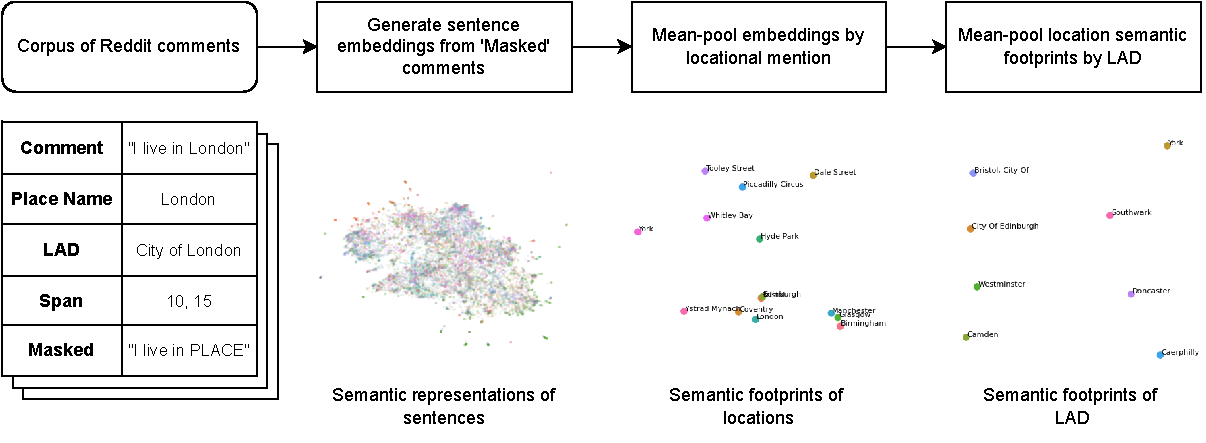
\includegraphics{./figures/workflow.pdf}

}

\caption{\label{fig-workflowfoot}Workflow diagram showing Reddit Corpus
processed into sentence embeddings, then aggregated into location and
LAD semantic footprints.}

\end{figure}%

Given each \(LAD\) has a variable number of comments associated with
them, we must process associated embeddings into a `semantic footprint'
representation of a fixed size, so that they may be directly compared.
To achieve this, all embeddings associated with comments relating to
locations within a \(LAD_j\) are processed into a one-dimension vector
of size \(1x768\). The most common approach for this dimensionality
reduction uses `mean-pooling'; taking the mean across all embeddings,
which is common in tasks like topic analysis (Reimers and Gurevych,
2019).

By masking place names, we ensure that no comment embeddings
accidentally incorporate geographically grounded information. For
example, comments in South Eastern local authorities are likely to
frequently mention London, given they are geographically proximal.
Embeddings for these locations would therefore capture an association
through the mention of London, rather than general semantic information.
For our work, we want to exclude any geographic information, ensuring
that embeddings solely capture semantic associations.

Given that transformers are a relatively new architecture in natural
language processing, and the creation of these models require
significant computational resources and training time, their use to date
has been limited in related research. Our choice to use the transformer
architecture stems from the emphasis we place on the extraction of
nuanced and contextual semantic information, which is lost with lexical
count-based methods like TF-IDF. It should be noted however that while
TF-IDF methods are less complex, they are typically more interpretable;
for instance, words that contribute importance to an embedding may be
extracted from a TF-IDF model. The numerical representations of any text
generated by transformers are not directly interpretable in this manner.
The following section therefore analyses our semantic footprints with
respect to their numerical representations, rather than through their
lexicons.

\subsection{Spatial Clustering and
Autocorrelation}\label{spatial-clustering-and-autocorrelation}

It is reasonable to assume that there are LADs within our corpora that
generate embeddings that capture similar semantic properties. A typical
method to group unlabelled multi-variate data based on shared properties
uses unsupervised clustering (Likas, Vlassis and J. Verbeek, 2003;
Sinaga and Yang, 2020). Therefore, to explore whether geographically
cohesive clusters appear within our semantic embeddings, we generate
hierarchical clusters, which are non-geographically bounded, using
agglomerative clustering. This clustering method allows for the optimal
number of clusters to be determined automatically, which was determined
to be 3. These clusters were visualised geographically, to examine
whether geographically cohesive groupings occurred. The proportion of
clusters present within each administrative region (RGN)\footnote{The
  highest tier of sub-national division in England. For Scotland and
  Wales we use the full national extents.} in Great Britain was also
plotted to determine whether clusters appeared to correlate with
administrative boundaries.

To quantify the level of spatial autocorrelation that our embeddings
exhibit, we consider the Moran's I metric, which identifies the spatial
relationship between each observation and its geographic neighbours
(Anselin, 1995; Rey, Arribas-Bel and Wolf, 2023). Moran's I values are
generated based on the strength of correlation between values and the
aggregate values of their geographic neighbours, known as their spatial
lag. Higher Moran's I values therefore denote a stronger spatial
autocorrelation. Given that Moran's I analysis requires univariate data,
we explore global spatial autocorrelation of our semantic footprints
UMAP decomposed into two dimensions, and plot both dimensions against
their spatial lag, giving two distinct global Moran's I values.

We then consider how localised levels of high spatial autocorrelation
may be identified through a Local Indicators of Spatial Autocorrelation
(LISA) analysis. Instead of single global values, LISA analysis
determines whether each unique LAD polygon exhibits a significant level
of spatial autocorrelation, and assigns a local Moran's I value for
each.

It is important to note that the magnitude of our embeddings do not
convey any definable information, values therefore only highlight
differences in semantic information between regions, rather than
importance. For example, an embedding value of 0 is not less important
than a value of 1 or -1.

\subsection{Semantic Similarity}\label{semantic-similarity}

Following our analysis of LAD semantic footprints, we explore our
semantic footprints from a top-down perspective, aggregating LADs into
established large-scale RGNs across Great Britain, taking the mean of
the collective semantic footprints. Each RGN is therefore represented by
a single 768 dimension semantic footprint embedding. We then calculate
the cosine similarity between each RGN embedding, demonstrating the
level of inter-region semantic cohesion across Great Britain.

Cosine similarity is a common metric for comparing embeddings, as it is
invariant to the magnitude of the vectors, and only considers the
direction. This is important as the magnitude of embeddings is not
meaningful, and only the direction of the vector conveys information.
For example, the embedding for the `South East' cannot be twice as
important as the embedding for the `North West'.

\subsection{Capturing National Identities through
Text}\label{capturing-national-identities-through-text}

To generate explainable characteristics of any geographically distinct
semantic footprints generated in our analysis, we consider how a
language model associates national identities with the semantic
properties of text. In our approach we mirror qualitative data
collection methodologies in political science research, where
individuals are typically queried as to their chosen national identity
(Haesly, 2005; Griffiths, 2022), instead generating the categorisations
of comments by querying a large language model (LLM).

LLMs are pre-trained on a large corpus of natural language text,
building representations of this text that emulate a human understanding
of language. The underlying theory is that these representations capture
the collective knowledge of humans that contributed the natural language
text used to build them. Therefore, in addition to factual information,
when posed with non-deterministic questioning, these models are able to
contribute the biased information that is incorporated into their model
weights.

Recent research has noted on the ability to perform zero-shot
classification using LLMs, where class predictions may be made without
the model ever having previously seen the labels (Wei, Bosma, \emph{et
al.}, 2022; Wei, Tay, \emph{et al.}, 2022). While research has
considered the use of questionnaires to query the strength of national
identities within the UK (Haesly, 2005; Griffiths, 2022), an LLM may
instead be used. For example, an LLM may be questioned whether it
personally feels a sequence of text appears to be `British', `English',
`Scottish', or `Welsh'. Through this zero-shot classification, we are
able to determine the strength of national identity associated with each
region in our work, to examine whether this appears to correlate with
any cohesion between the semantic footprints that we generate.
Importantly, we are also able to generate confidence values from the
chosen LLM, allowing for the strength of these national identities to be
captured.

Semantic information within our comments is expected to capture both
explicit information contributed by users; for example stating `London
is a British city', in addition to implicit semantic information that
exists within language. For example the phrase `bonnie Scotland' may
suggest a strong identity due to the inclusion of Scottish
slang\footnote{See `Scottish English' or `Scots'; (Stuart-Smith, 2008)}.
Unlike our semantic footprints, we do not mask place name mentions in
these embeddings, enabling the model to make its own decisions regarding
place name mentions.

To identify regional identities through semantic information, we build
on the emergent properties of large language models, which enable a task
known as `Zero-Shot Classification'. This allows models to predict a
class that was not seen during training, by generating a prompt that
contains the labels required. For this task we select the
\texttt{typeform/distilbert-base-uncased-mnli} model\footnote{https://huggingface.co/typeform/distilbert-base-uncased-mnli},
which is tailored towards zero-shot classification, therefore generating
slightly different embeddings compared with those used for our semantic
footprints. For our task the following gives an example prompt with a
portion of a comment taken from our corpus, where the Scottish
colloquial slang `gonnae' is used:

\begin{verbatim}
Classify the following input text into one of the following four categories:
[British, English, Scottish, Welsh]

Input Text: My favourite was in Livingston: 'Rab, I'm gonnae find you.'
\end{verbatim}

The output would then be given as a sequence of confidence values for
each label:

\begin{verbatim}
'labels': ['Scottish', 'British', 'Welsh', 'English']
'scores': [0.761, 0.144, 0.052, 0.043]
\end{verbatim}

\section{Results}\label{sec-results}

\begin{figure}

\centering{

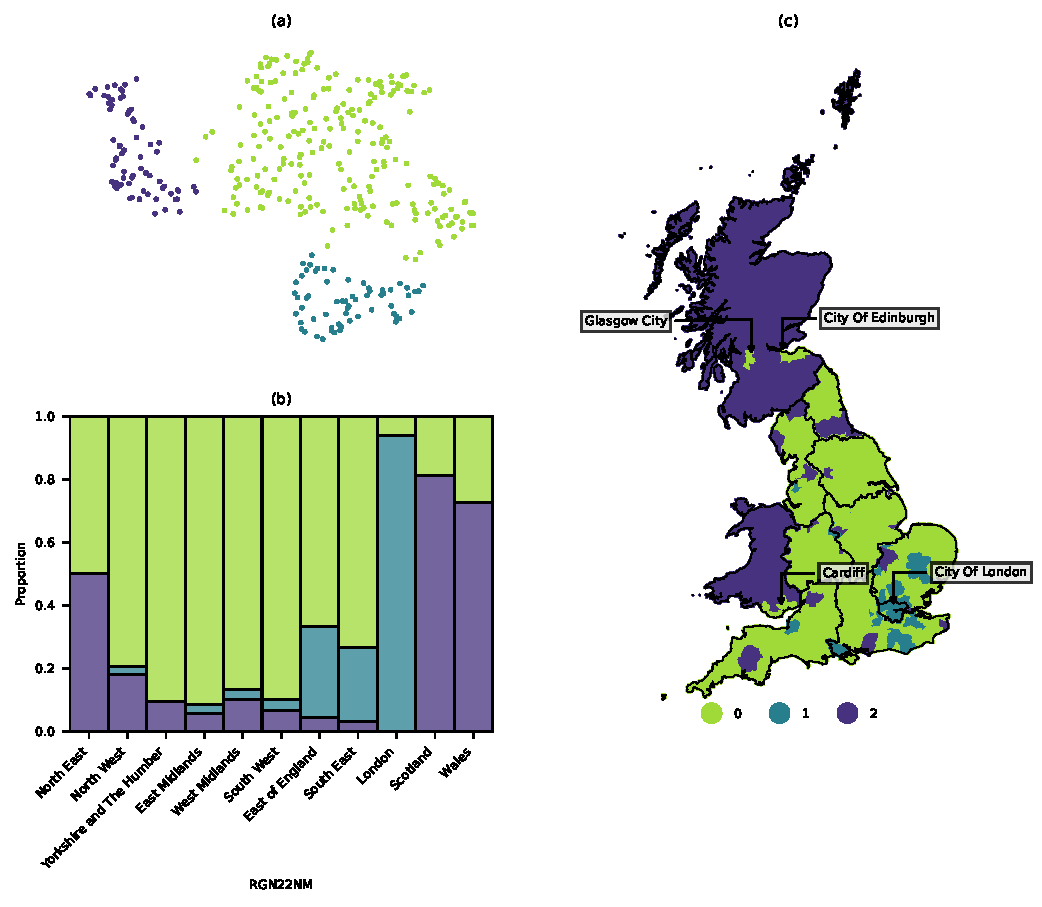
\includegraphics{main_files/figure-pdf/fig-clusters-output-1.pdf}

}

\caption{\label{fig-clusters}Semantic footprints associated with each
LAD corpus coloured by hierarchical agglomerative clusters where
\(K=3\). (a) Footprints UMAP decomposed into two dimensions. (b)
Proportion of clusters by RGN. (c) Geographic location of clusters.}

\end{figure}%

Figure~\ref{fig-clusters} (a) shows clusters of LAD transformer
embeddings UMAP decomposed into two dimensions, indicating embeddings
that share similar semantic properties. These clusters appear to broadly
correlate with three distinct regions within Great Britain, where
cluster 0 most closely identifies with England, 1 with London and
surrounding areas, and 2 with Scotland and Wales
(Figure~\ref{fig-clusters} (b-c)). The few areas that appear as cluster
0 in Wales and Scotland are major urban centres like Cardiff, Glasgow,
and Edinburgh. Overall these clusters appear to be geographically
restricted, and even broadly conform with administrative regions like
the Welsh and Scottish borders.

These findings appear to share similarities with past work that has
observed strong `boundary effects', where lexical similarity between
geotagged Tweets often correlates with administrative boundaries (Yin
\emph{et al.}, 2017; Bailey \emph{et al.}, 2018; Arthur and Williams,
2019; Li \emph{et al.}, 2021). Our embeddings also exhibit the general
geographically coherent patterns that have been observed in geographical
lexical variations in social media (Russ, 2012; Doyle, 2014; Gonçalves
and Sánchez, 2014; Eisenstein \emph{et al.}, 2014; Huang \emph{et al.},
2016; Pérez \emph{et al.}, 2019; Arthur and Williams, 2019). Notably,
unlike dialects, where a geographic component is expected, the
geographic association of our general semantic embeddings has not been
demonstrated in past work. Results therefore demonstrate that despite no
pre-existing geographic information like geotags or place names, general
text associated with locations appears to embed a geographic component.
The geographic coherence in our results is particularly strong at the
borders of Scotland and Wales, which conforms with our hypothesis that
the vernacular geography that exists within social media text embeds
components that contribute to the strength of national identities
(Haesly, 2005).

As noted however, major cities in Wales and Scotland Glasgow, Edinburgh
and Cardiff share a cluster with English LADs rather than their
respective country, suggesting that these locations are more
semantically connected with the rest of Great Britain. This observation
mirrors the results of work that considered co-occurring locational
mentions between cities, where shared city mentions in text often appear
irrespective of distance, and across administrative borders
{[}anonymised{]}. This deviation from the relative semantic isolation of
Scotland and Wales from England appears to be reflective of the nature
of major cities, given they tend to share stronger physical geographic
connections across a larger geographic scope, and more influential
cultural connections compared with rural areas, captured in our work
through shared semantic traits.

Cluster 1 presents in areas surrounding London and suggests
distinctiveness of this region relative to the rest of Great Britain.
This is interesting given London's extensive connectivity relative to
the rest of the country, and the general sense of strong association
with other cities, given it is the capital city {[}anonymised{]}. Our
results therefore suggest that despite London's importance nationally,
semantic information is able to capture a deeper context that
dissociates it from other regions. This effect may be due to factors
unique to London, for example its prominence globally, influencing both
tourism and business external to the United Kingdom, which alter the
cultural landscape of the city. The isolated characteristics of London
are particularly observable through its economic differences, where high
costs of living have generated the need for a `London
weighting'\footnote{https://en.wikipedia.org/wiki/London\_weighting} of
salaries (Hirsch, 2016).

The following section formalises the level of geographic coherence that
the embeddings exhibit, and highlights the key locations that drive the
relationship between text and geography.

\subsection{Moran's I Analysis}\label{morans-i-analysis}

\begin{figure}

\centering{

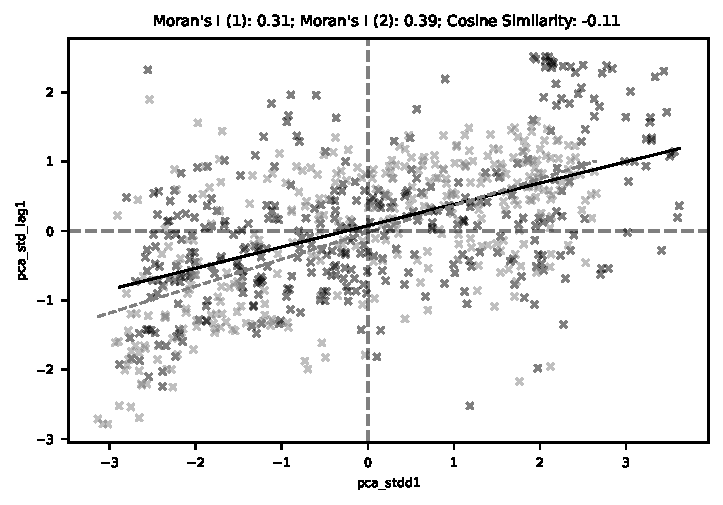
\includegraphics{main_files/figure-pdf/fig-morans-output-1.pdf}

}

\caption{\label{fig-morans}Moran's I Plot: LAD embeddings decomposed
into 2 dimensions and standardised against their spatial lag.}

\end{figure}%

To quantify whether our embeddings demonstrate spatial autocorrelation,
we consider the Moran's I metric, which identifies the spatial
relationship between each observation and its geographic neighbours
(Anselin, 1995). Given that this analysis requires univariate data, we
explore global spatial autocorrelation of our UMAP decomposed embeddings
computing the spatial lag for both dimensions. On
Figure~\ref{fig-morans}, we plot both values for each LAD semantic
footprint in Great Britain, against the spatial lag of these values. A
higher correlation between the semantic footprints values and their
spatial lag indicates a stronger level of global spatial
autocorrelation, resulting in a higher Moran's I value.
Figure~\ref{fig-morans} shows a positive correlation between the PCA
decomposed embedding values and their spatial lag, resulting in Moran's
I values of 0.31 and 0.39. This indicates a reasonably strong spatial
autocorrelation with both embedding dimensions, confirming that semantic
footprints are typically more similar between nearby locations. While
the Moran's I values for both dimensions are similar, their cosine
similarity is negative (-0.11), meaning these two decomposed dimensions
capture distinctly different semantic traits.

While spatially coherent results have been demonstrated from the
perspective of dialects on social media (Russ, 2012; Doyle, 2014;
Gonçalves and Sánchez, 2014; Eisenstein \emph{et al.}, 2014; Huang
\emph{et al.}, 2016; Pérez \emph{et al.}, 2019; Arthur and Williams,
2019), we have demonstrated that this phenomenon can also be captured
from general semantic information. Notably, while dialects have always
been considered to have strong geographical grounding (Trudgill, 2004),
it is more surprising that general semantic information regarding
locations similarly exhibits this relationship.

\begin{figure}

\centering{

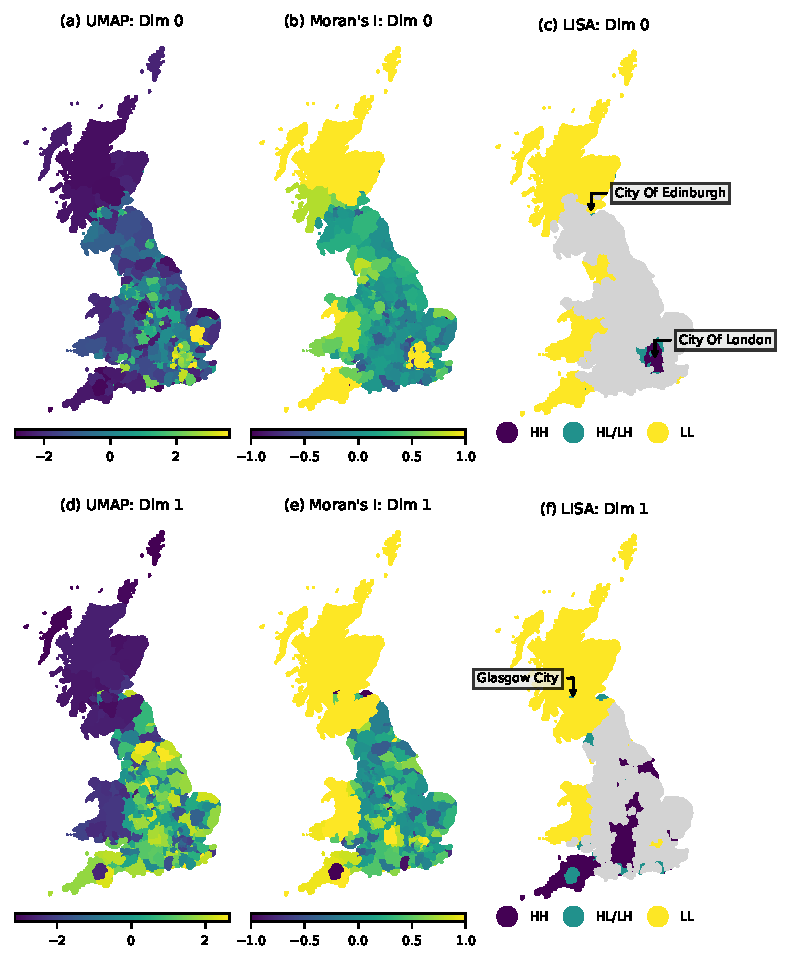
\includegraphics{main_files/figure-pdf/fig-lisa-output-1.pdf}

}

\caption{\label{fig-lisa}Local Indicators of Spatial Auto-correlation
(LISA). (a/d) 1 dimensional embedding values. (b/e) Local Moran's I
values (\(Is\)). (c/f) LISA HH and LL significant values (\(p<0.05\)),
both are included as the value of embeddings do not convey information.}

\end{figure}%

To explore local indicators of spatial autocorrelation (LISA) we plot
each decomposed embedding on Figure~\ref{fig-lisa} (a/d), each local
Moran's I value on (b/e) and all significant (\(p<0.05\)) HH and LL LISA
quadrants on (c/f). Note that only selecting significant \(p\) values on
Figure~\ref{fig-lisa} (c/f) ensures that no regions are included that
have values that could demonstrate autocorrelation even if randomly
distributed geographically. From Figure~\ref{fig-lisa} (c/f), we can see
that notable large areas with significant levels of spatial correlation
include;

\begin{itemize}
\tightlist
\item
  Scotland
\item
  Wales
\item
  London and surrounding LADs
\item
  the South West; towards Cornwall
\end{itemize}

As demonstrated by the low cosine similarity between our UMAP
embeddings, they appear to capture distinctly different semantic
information. London for example only appears in dimension 0, while
dimension 1 captures broader spatial autocorrelation across Scotland and
Wales. In Scotland we can see that from both LISAs, Glasgow and
Edinburgh represent areas of HL/LH, where semantic information in these
cities is not the same as surrounding LADs, an effect that is also
captured in some LADs surrounding London. England overall appears to be
a less semantically cohesive country based on this analysis, where most
LADs do not contribute significant levels of spatial autocorrelation.

These results again demonstrate geographic cohesion between semantic
footprints, which notably appear to correspond with the national
boundaries of Wales and Scotland. This mirrors the observations of past
work where dialect differences appeared to correlate with administrative
boundaries (Yin \emph{et al.}, 2017; Bailey \emph{et al.}, 2018; Arthur
and Williams, 2019; Li \emph{et al.}, 2021). In addition to Wales and
Scotland, we have also identified a notable grouping in the South West,
which potentially reflects the Cornish identity (Deacon, 2007), as well
as a grouping associated with London.

\subsection{Semantic Similarity and
Identity}\label{semantic-similarity-and-identity}

\begin{figure}

\centering{

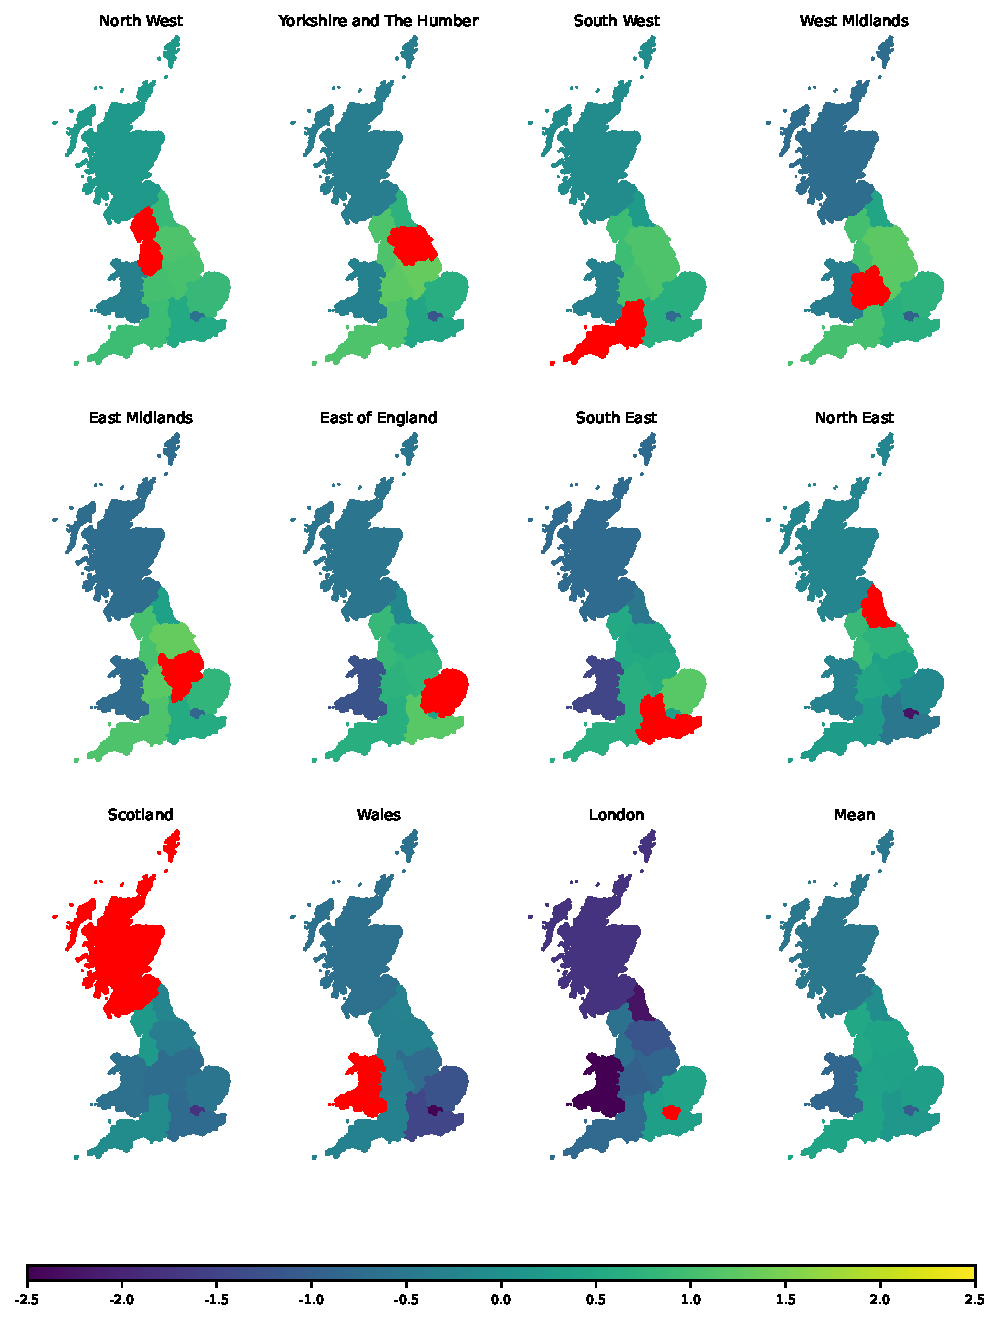
\includegraphics{main_files/figure-pdf/fig-similarity-output-1.pdf}

}

\caption{\label{fig-similarity}Scaled cosine similarity of embeddings
for administrative regions across the UK. Higher values indicate greater
cosine similarity. Regions shown in descending order by mean cosine
similarity value.}

\end{figure}%

Given the regions highlighted as having strong spatial autocorrelation
in their semantic footprints appear to broadly conform with the
administrative regions of Wales, Scotland, and London, we examine these
footprints from a top-down analysis using pre-defined larger scale
aggregations.

Figure~\ref{fig-similarity} compares the cosine similarity between each
RGN embedding, allowing for inter-regional cohesion to be explored. The
North West has the overall highest level of cosine similarity,
displaying comparatively high similarity with most regions across
England, excluding London. London has the lowest overall similarity,
only sharing positive cosine similarity values with the South and South
East of England. As expected, Scotland and Wales have low overall cosine
similarity values, with Wales sharing even lower similarity with respect
to London and the South East compared with Scotland. Mean values show
clearly that the least cohesive regions appear to be London, Wales, and
Scotland, three regions that are also those with the strongest levels of
spatial autocorrelation.

Excluding London, the North East is the region in England with the
lowest overall cosine similarity with the rest of Great Britain. This is
perhaps reflective of distinct differences with this region, for example
the distinctly lower gross value added (GVA) compared with other regions
(Fenton, 2018), or the general sense of strong identity that is often
noted by residents (Middleton and Freestone, 2008). Alternatively, the
North West is home to nationally influential urban conurbations,
especially between Manchester and Liverpool (Oguz and Walton, 2022),
likely generating the highest overall semantic similarity of this region
compared with the rest of the UK. Comparatively, the East of England,
South East and London are neighbouring regions that share high
similarities with each other, but exhibit low similarity with the rest
of Great Britain, suggesting there are semantic components that
distinguish this region of the country from the rest. There is a
slightly higher mean similarity with respect to Scotland compared with
Wales, due to higher similarities with regions in England, like the
North West and South East. Major urban centres in Scotland are
relatively well connected to Great Britain through rail routes, and
Edinburgh and Glasgow are historically important UK cities, captured by
their distinct difference in embedding values during the spatial
autocorrelation analysis. This factor likely increases the cosine
similarity of Scotland with regions in England, while Wales in this
sense is less directly associated with the rest of the UK.

To determine whether regional identities generated by a large language
model aligns with these semantically isolated regions in our analysis,
we plot the distribution of regional identities identified through our
zero-shot classification on Figure~\ref{fig-identity}.

Across each region, the `English' identity is always lower than
`British', suggesting that regions within England are typically more
strongly associated with the United Kingdom\footnote{Note that despite
  etymologically relating to `Great Britain', the term `British' refers
  to `belonging to or relating to the United Kingdom of Great Britain
  and Northern Ireland'} than solely England. Unlike English regions
however, comments relating to both Scottish and Welsh locations are more
strongly associated with their respective nationalities. However,
comments relating to Welsh locations appear on average to have stronger
confidence values with respect to the British classification, compared
with Scottish locations. Similar observations have been captured from
qualitative interviewing, where Welsh residents similarly appear to more
strongly associate themselves with the British identity, compared with
Scottish residents (Haesly, 2005; Llamas, 2009; Carman, Johns and
Mitchell, 2014; Llamas and Watt, 2014). Of the English regions, London
has a distinctly higher average confidence value of both British and
English identities compared with all other regions. Notably given the
semantic footprints for Scotland, Wales, and London also have the lowest
overall cosine similarity values, these differences in generated
identity compared with other regions are a likely component in their
semantic differences.

\begin{figure}

\centering{

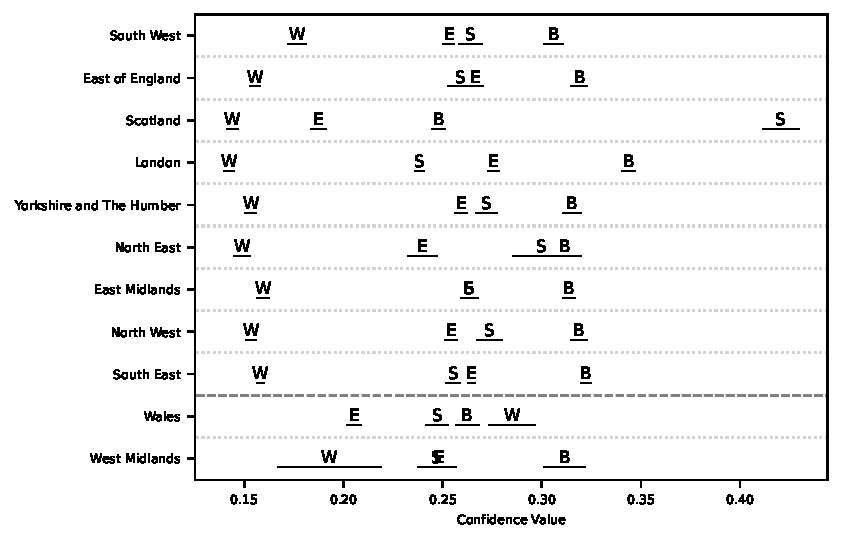
\includegraphics{main_files/figure-pdf/fig-identity-output-1.pdf}

}

\caption{\label{fig-identity}Zero Shot classification of each corpus
into regional identities; {[}B{]}ritish, {[}E{]}nglish, {[}S{]}cottish,
{[}W{]}elsh. Values show mean confidence value across each comment,
lines indicate standard error. Descending order by {[}B{]}ritish
confidence. The dashed line separates English regions from Scotland and
Wales.}

\end{figure}%

\subsection{General Observations}\label{general-observations}

Unlike typical representations of the North-South divide within England
(Jewell, 1994), semantic differences appear to be influenced primarily
by proximity to London. Unlike typical representations of this divide,
the South West of England therefore appears to be distinct from the
South East, with a stronger association with the North. South Eastern
regions however do share lower similarity to the Midlands and North of
England, which conforms with a typical view of the English North-South
divide.

In a similar sense, Scotland and Wales demonstrate distinctly more
cohesive semantic properties compared with England, where groupings of
high spatial autocorrelation are constrained to smaller regions, like
London. In traditional linguistic research, the spoken dialect across
England is known to vary considerably (Knowles, 1973; Chambers and
Trudgill, 1998; Deacon, 2007; MacKenzie, Bailey and Turton, 2022), which
itself captures the distinct social differences, and the localised
identities that exist across geographic space. Instead, the high
cohesion within Wales and Scotland appears to capture the sense of
national identity that these constituent countries exhibit in our
analysis, and is a common qualitative observation in political science
research (Haesly, 2005; Carman, Johns and Mitchell, 2014).

As demonstrated in past work that has examined both physical and
non-physical networks, our observed semantic information similarly
appears to correlate with pre-defined administrative boundaries,
particularly the national boundaries of Scotland and Wales (Yin \emph{et
al.}, 2017; Bailey \emph{et al.}, 2018; Arthur and Williams, 2019; Li
\emph{et al.}, 2021). The distinct difference in footprints between each
constituent country in the UK conforms with the idea that vernacular
geography captures a sense of identity, given our zero-shot
classification demonstrates distinct nationalities between Scotland and
Wales, unlike English regions where the generated national identity is
typically considered British rather than English. Notably however, the
slightly stronger British identity within Wales has been observed
previously through qualitative interviewing (Haesly, 2005; Carman, Johns
and Mitchell, 2014), suggesting that even the nuanced properties of text
appear to correlate with the true perceptions of individuals. It is also
worth noting that, given the exclusion of place names in our embeddings,
these distinct differences are not simply the result of differences in
place names (e.g.~place names in Wales are distinct from England), which
may have influenced the results of past lexical work.

Despite most locations across Scotland and Wales appearing disconnected
with the rest of the UK, major cities like Glasgow and Edinburgh are
more semantically similar, a distinction that was also observed when the
distance decay of locational co-occurrences in text was examined
{[}anonymised{]}. This suggests that these cities do appear to be
typically more semantically connected with the UK, regardless of
geographic distance and borders, while other locations typically share
semantic properties within the same nation, captured through stronger
spatial autocorrelation.

Internal migration patterns within the UK are primarily influenced by
family ties, rather than economic factors, employment, or education
(Thomas, 2019). The observations made in our work demonstrate that this
sense of belonging to regions influences the geographically cohesive
nature of our semantic footprints. While populations have the ability to
distribute evenly across geographic space, they are often reluctant to
move far. Local inhabitants within regions develop an identity
associated with their home region, traditionally captured in language
through dialect variation, and demonstrated in our work through broader
semantic associations, which embed contextual meaning, incorporating the
cultural variation of regions.

\section{Conclusion}\label{sec-conclusion}

Our paper demonstrates a new method to compare aggregate semantic
information for local authorities and regions within the UK, from Reddit
comments that mention geoparsed locations, which we name semantic
footprints. When examining the semantic footprints of each LAD in the
UK, we find that geographically cohesive clusters appear, with
significant levels of spatial autocorrelation. Clusters broadly conform
with the national borders of Scotland and Wales, while London also
appears to be semantically distinct from the rest of England. Through an
examination of generated national identities associated with each
region, we find that these distinct geographic groupings are a likely
result of associated identities, which are generated through general
associations captured through the vernacular geography of all users in
our social media corpus.

Geoparsing methods contribute an additional geographic dimension to
non-geotagged social media data, allowing for a much larger repository
of informal natural language geographic text to be used for research.
Future work may consider the use of Reddit comment data to derive
notable urban areas of interest (Chen, 2019). This area of research in
particular would benefit from methodologies focussing on the extraction
of fine-grained locations from text, which at present is a challenging
task (Han \emph{et al.}, 2018).

\section*{References}\label{references}
\addcontentsline{toc}{section}{References}

\phantomsection\label{refs}
\begin{CSLReferences}{0}{1}
\bibitem[\citeproctext]{ref-agnew2005}
Agnew, J. (2005) {`Space: Place in {Cloke P} and {Johnston R} eds
{Spaces} of geographical thought'}.

\bibitem[\citeproctext]{ref-anselin1995}
Anselin, L. (1995) {`Local {Indicators} of {Spatial
Association}{\textemdash}{LISA}'}, \emph{Geographical Analysis}, 27(2),
pp. 93--115. Available at:
\url{https://doi.org/10.1111/j.1538-4632.1995.tb00338.x}.

\bibitem[\citeproctext]{ref-arthur2019}
Arthur, R. and Williams, H.T.P. (2019) {`The human geography of
{Twitter}: {Quantifying} regional identity and inter-region
communication in {England} and {Wales}'}, \emph{PLOS ONE}. Edited by E.
Ferrara, 14(4), p. e0214466. Available at:
\url{https://doi.org/10.1371/journal.pone.0214466}.

\bibitem[\citeproctext]{ref-bailey2018}
Bailey, M. \emph{et al.} (2018) {`Social {Connectedness}: {Measurement},
{Determinants}, and {Effects}'}, \emph{Journal of Economic
Perspectives}, 32(3), pp. 259--280. Available at:
\url{https://doi.org/10.1257/jep.32.3.259}.

\bibitem[\citeproctext]{ref-baumgartner2020}
Baumgartner, J. \emph{et al.} (2020) {`The {Pushshift Reddit Dataset}'}.
{arXiv}. Available at: \url{https://arxiv.org/abs/2001.08435} (Accessed:
18 May 2022).

\bibitem[\citeproctext]{ref-berragan2023a}
Berragan, C. \emph{et al.} (2023) {`Transformer based named entity
recognition for place name extraction from unstructured text'},
\emph{International Journal of Geographical Information Science}, 37(4),
pp. 747--766. Available at:
\url{https://doi.org/10.1080/13658816.2022.2133125}.

\bibitem[\citeproctext]{ref-buttimer2015}
Buttimer, A. (2015) {`Home, reach, and the sense of place'}, in
\emph{The human experience of space and place}. {Routledge}, pp.
166--187.

\bibitem[\citeproctext]{ref-carman2014}
Carman, C., Johns, R. and Mitchell, J. (2014) \emph{More {Scottish} than
{British}: {The} 2011 {Scottish Parliament Election}}. {Springer}.

\bibitem[\citeproctext]{ref-chambers1998}
Chambers, J.K. and Trudgill, P. (eds) (1998) {`Social differentiation
and language'}, in \emph{Dialectology}. 2nd edn. {Cambridge}: {Cambridge
University Press} (Cambridge {Textbooks} in {Linguistics}), pp. 57--69.
Available at: \url{https://doi.org/10.1017/CBO9780511805103.007}.

\bibitem[\citeproctext]{ref-chen2019}
Chen, M. (2019) {`Understanding the dynamics of urban areas of interest
through volunteered geographic information'}, p. 21. Available at:
\url{https://doi.org/10.1007/s10109-018-0284-3}.

\bibitem[\citeproctext]{ref-daniel2007}
Daniel, J. and James H, M. (2007) \emph{Speech and language processing:
{An} introduction to natural language processing, computational
linguistics, and speech recognition}. {prentice hall}.

\bibitem[\citeproctext]{ref-deacon2007}
Deacon, B. (2007) {`County, {Nation}, {Ethnic Group}? {The Shaping} of
the {Cornish Identity}'}, \emph{The International Journal of Regional
and Local Studies}, 3(1), pp. 5--29. Available at:
\url{https://doi.org/10.1179/jrl.2007.3.1.5}.

\bibitem[\citeproctext]{ref-devlin2019}
Devlin, J. \emph{et al.} (2019) {`{BERT}: {Pre-training} of {Deep
Bidirectional Transformers} for {Language Understanding}'},
\emph{arXiv:1810.04805 {[}cs{]}} {[}Preprint{]}. Available at:
\url{https://arxiv.org/abs/1810.04805} (Accessed: 11 February 2020).

\bibitem[\citeproctext]{ref-doyle2014}
Doyle, G. (2014) {`Mapping {Dialectal Variation} by {Querying Social
Media}'}, in \emph{Proceedings of the 14th {Conference} of the {European
Chapter} of the {Association} for {Computational Linguistics}}.
{Gothenburg, Sweden}: {Association for Computational Linguistics}, pp.
98--106. Available at: \url{https://doi.org/10.3115/v1/E14-1011}.

\bibitem[\citeproctext]{ref-eisenstein2014}
Eisenstein, J. \emph{et al.} (2014) {`Diffusion of {Lexical Change} in
{Social Media}'}, \emph{PLoS ONE}. Edited by R.C. Berwick, 9(11), p.
e113114. Available at:
\url{https://doi.org/10.1371/journal.pone.0113114}.

\bibitem[\citeproctext]{ref-evans2007}
Evans, A.J. and Waters, T. (2007) {`Mapping vernacular geography:
Web-based {GIS} tools for capturing 'fuzzy' or 'vague' entities'},
\emph{International Journal of Technology, Policy and Management}
{[}Preprint{]}.

\bibitem[\citeproctext]{ref-fenton2018}
Fenton, T. (2018) {`Regional economic activity by gross value added
(balanced), {UK} - {Office} for {National Statistics}'}.
https://www.ons.gov.uk/economy/grossvalueaddedgva/bulletins/regionalgrossvalueaddedbalanceduk/1998to2017.

\bibitem[\citeproctext]{ref-gao2017a}
Gao, S. \emph{et al.} (2017) {`A data-synthesis-driven method for
detecting and extracting vague cognitive regions'}, \emph{International
Journal of Geographical Information Science}, 31(6), pp. 1245--1271.
Available at: \url{https://doi.org/10.1080/13658816.2016.1273357}.

\bibitem[\citeproctext]{ref-goncalves2014}
Gonçalves, B. and Sánchez, D. (2014) {`Crowdsourcing {Dialect
Characterization} through {Twitter}'}, \emph{PLoS ONE}. Edited by T.
Preis, 9(11), p. e112074. Available at:
\url{https://doi.org/10.1371/journal.pone.0112074}.

\bibitem[\citeproctext]{ref-goodchild2011}
Goodchild, M.F. and Li, L. (2011) {`Formalizing space and place'}.

\bibitem[\citeproctext]{ref-griffiths2022}
Griffiths, J.D. (2022) {`Scrutinizing {Relative Territorial Identity
Measures}'}, \emph{Publius: The Journal of Federalism}, 53(1), pp.
133--151. Available at: \url{https://doi.org/10.1093/publius/pjac011}.

\bibitem[\citeproctext]{ref-haesly2005}
Haesly, R. (2005) {`Identifying {Scotland} and {Wales}: Types of
{Scottish} and {Welsh} national identities'}, \emph{Nations and
Nationalism}, 11(2), pp. 243--263. Available at:
\url{https://doi.org/10.1111/j.1354-5078.2005.00202.x}.

\bibitem[\citeproctext]{ref-han2012}
Han, B., Cook, P. and Baldwin, T. (2012) {`Geolocation {Prediction} in
{Social Media Data} by {Finding Location Indicative Words}'}, p. 18.

\bibitem[\citeproctext]{ref-han2018}
Han, J. \emph{et al.} (2018) {`Linking {Fine-Grained Locations} in {User
Comments}'}, \emph{IEEE Transactions on Knowledge and Data Engineering},
30(1), pp. 59--72. Available at:
\url{https://doi.org/10.1109/TKDE.2017.2758780}.

\bibitem[\citeproctext]{ref-hirsch2016}
Hirsch, D. (2016) {`London weighting and {London} costs-a fresh
approach?'}

\bibitem[\citeproctext]{ref-hollenstein2008}
Hollenstein, L. (2008) {`Capturing vernacular geography from
georeferenced tags'}.

\bibitem[\citeproctext]{ref-hu2020}
Hu, S. \emph{et al.} (2020) {`A framework for extracting urban
functional regions based on multiprototype word embeddings using
points-of-interest data'}, \emph{Computers, Environment and Urban
Systems}, 80, p. 101442. Available at:
\url{https://doi.org/10.1016/j.compenvurbsys.2019.101442}.

\bibitem[\citeproctext]{ref-huang2016}
Huang, Y. \emph{et al.} (2016) {`Understanding {U}.{S}. Regional
linguistic variation with {Twitter} data analysis'}, \emph{Computers,
Environment and Urban Systems}, 59, pp. 244--255. Available at:
\url{https://doi.org/10.1016/j.compenvurbsys.2015.12.003}.

\bibitem[\citeproctext]{ref-jewell1994}
Jewell, H.M. (1994) \emph{The {North-south Divide}: {The Origins} of
{Northern Consciousness} in {England}}. {Manchester University Press}.

\bibitem[\citeproctext]{ref-knowles1973}
Knowles, G.O. (1973) {`Scouse: The urban dialect of {Liverpool}'}.

\bibitem[\citeproctext]{ref-kropczynski2018}
Kropczynski, J. \emph{et al.} (2018) {`Identifying {Actionable
Information} on {Social Media} for {Emergency Dispatch}'}, p. 11.

\bibitem[\citeproctext]{ref-lambiotte2008}
Lambiotte, R. \emph{et al.} (2008) {`Geographical dispersal of mobile
communication networks'}, \emph{Physica A: Statistical Mechanics and its
Applications}, 387(21), pp. 5317--5325. Available at:
\url{https://doi.org/10.1016/j.physa.2008.05.014}.

\bibitem[\citeproctext]{ref-lengyel2015}
Lengyel, B. \emph{et al.} (2015) {`Geographies of an {Online Social
Network}'}, \emph{PLOS ONE}. Edited by W.-X. Zhou, 10(9), p. e0137248.
Available at: \url{https://doi.org/10.1371/journal.pone.0137248}.

\bibitem[\citeproctext]{ref-li2021}
Li, Z. \emph{et al.} (2021) {`Measuring global multi-scale place
connectivity using geotagged social media data'}, \emph{Scientific
Reports}, 11(1), p. 14694. Available at:
\url{https://doi.org/10.1038/s41598-021-94300-7}.

\bibitem[\citeproctext]{ref-likas2003}
Likas, A., Vlassis, N. and J. Verbeek, J. (2003) {`The global k-means
clustering algorithm'}, \emph{Pattern Recognition}, 36(2), pp. 451--461.
Available at: \url{https://doi.org/10.1016/S0031-3203(02)00060-2}.

\bibitem[\citeproctext]{ref-llamas2009}
Llamas, C. (2009) \emph{Language and {Identities}}. {Edinburgh
University Press}.

\bibitem[\citeproctext]{ref-llamas2014}
Llamas, C. and Watt, D. (2014) {`Scottish, {English}, {British}?:
{Innovations} in {Attitude Measurement}'}, \emph{Language and
Linguistics Compass}, 8(11), pp. 610--617. Available at:
\url{https://doi.org/10.1111/lnc3.12109}.

\bibitem[\citeproctext]{ref-mackenzie2022}
MacKenzie, L., Bailey, G. and Turton, D. (2022) {`Towards an updated
dialect atlas of {British English}'}, \emph{Journal of Linguistic
Geography}, 10(1), pp. 46--66. Available at:
\url{https://doi.org/10.1017/jlg.2022.2}.

\bibitem[\citeproctext]{ref-middleton2008}
Middleton, C. and Freestone, P. (2008) {`The {Impact} of {Culture-led
Regeneration} on {Regional Identity} in {North East England}'}.

\bibitem[\citeproctext]{ref-murphy2019}
Murphy, N. (2019) {`Reddit's 2019 {Year} in {Review} - {Upvoted}'}.
https://www.redditinc.com/blog/reddits-2019-year-in-review/\#content.

\bibitem[\citeproctext]{ref-oguz2022}
Oguz, S. and Walton, A. (2022) {`Productivity in towns and travel to
work areas, {UK} - {Office} for {National Statistics}'}.
https://www.ons.gov.uk/economy/economicoutputandproductivity/publicservicesproductivity/articles/productivityintownsandtraveltoworkareasuk/2019.

\bibitem[\citeproctext]{ref-paasi2003}
Paasi, A. (2003) {`Region and place: Regional identity in question'},
\emph{Progress in human geography}, 27(4), pp. 475--485. Available at:
\url{https://doi.org/10.1191/0309132503ph439pr}.

\bibitem[\citeproctext]{ref-perez2019}
Pérez, J.M. \emph{et al.} (2019) {`Exploiting user-frequency information
for mining regionalisms from {Social Media} texts'}. {arXiv}. Available
at: \url{https://arxiv.org/abs/1907.04492} (Accessed: 23 May 2023).

\bibitem[\citeproctext]{ref-purves2019}
Purves, R.S., Winter, S. and Kuhn, W. (2019) {`Places in {Information
Science}'}, \emph{Journal of the Association for Information Science and
Technology}, 70(11), pp. 1173--1182. Available at:
\url{https://doi.org/10.1002/asi.24194}.

\bibitem[\citeproctext]{ref-rae2009}
Rae, A. (2009) {`From spatial interaction data to spatial interaction
information? {Geovisualisation} and spatial structures of migration from
the 2001 {UK} census'}, \emph{Computers, Environment and Urban Systems},
33(3), pp. 161--178. Available at:
\url{https://doi.org/10.1016/j.compenvurbsys.2009.01.007}.

\bibitem[\citeproctext]{ref-ratti2010}
Ratti, C. \emph{et al.} (2010) {`Redrawing the {Map} of {Great Britain}
from a {Network} of {Human Interactions}'}, \emph{PLoS ONE}. Edited by
O. Sporns, 5(12), p. e14248. Available at:
\url{https://doi.org/10.1371/journal.pone.0014248}.

\bibitem[\citeproctext]{ref-reades2009}
Reades, J., Calabrese, F. and Ratti, C. (2009) {`Eigenplaces: Analysing
cities using the space {\textendash} time structure of the mobile phone
network'}, \emph{Environment and Planning B: Planning and Design},
36(5), pp. 824--836. Available at:
\url{https://doi.org/10.1068/b34133t}.

\bibitem[\citeproctext]{ref-reimers2019}
Reimers, N. and Gurevych, I. (2019) {`Sentence-{BERT}: {Sentence
Embeddings} using {Siamese BERT-Networks}'}, in \emph{Proceedings of the
2019 {Conference} on {Empirical Methods} in {Natural Language
Processing} and the 9th {International Joint Conference} on {Natural
Language Processing} ({EMNLP-IJCNLP})}. {Hong Kong, China}: {Association
for Computational Linguistics}, pp. 3980--3990. Available at:
\url{https://doi.org/10.18653/v1/D19-1410}.

\bibitem[\citeproctext]{ref-rey2023}
Rey, S., Arribas-Bel, D. and Wolf, L.J. (2023) \emph{Geographic data
science with python}. {CRC Press}.

\bibitem[\citeproctext]{ref-russ2012}
Russ, B. (2012) {`Examining large-scale regional variation through
online geotagged corpora'}, in.

\bibitem[\citeproctext]{ref-sinaga2020}
Sinaga, K.P. and Yang, M.-S. (2020) {`Unsupervised {K-Means Clustering
Algorithm}'}, \emph{IEEE Access}, 8, pp. 80716--80727. Available at:
\url{https://doi.org/10.1109/ACCESS.2020.2988796}.

\bibitem[\citeproctext]{ref-sobolevsky2013}
Sobolevsky, S. \emph{et al.} (2013) {`Delineating {Geographical Regions}
with {Networks} of {Human Interactions} in an {Extensive Set} of
{Countries}'}, \emph{PLoS ONE}. Edited by Y. Moreno, 8(12), p. e81707.
Available at: \url{https://doi.org/10.1371/journal.pone.0081707}.

\bibitem[\citeproctext]{ref-statista2022}
Statista (2022) {`Most popular social networks worldwide as of {January}
2022, ranked by number of monthly active users'}, \emph{Statista}.
https://www.statista.com/statistics/272014/global-social-networks-ranked-by-number-of-users/.

\bibitem[\citeproctext]{ref-stuart-smith2008}
Stuart-Smith, J. (2008) {`Scottish {English}: {Phonology}'},
\emph{Varieties of English}, 1, pp. 48--70.

\bibitem[\citeproctext]{ref-sui2011}
Sui, D. and Goodchild, M.F. (2011) {`The convergence of {GIS} and social
media: Challenges for {GIScience}'}, \emph{International Journal of
Geographical Information Science}, 25(11), pp. 1737--1748. Available at:
\url{https://doi.org/10.1080/13658816.2011.604636}.

\bibitem[\citeproctext]{ref-thomas2019}
Thomas, M.J. (2019) {`Employment, education, and family: {Revealing} the
motives behind internal migration in {Great Britain}'},
\emph{Population, Space and Place}, 25(4), p. e2233. Available at:
\url{https://doi.org/10.1002/psp.2233}.

\bibitem[\citeproctext]{ref-titheridge2009}
Titheridge, H. \emph{et al.} (2009) {`Assessing the extent of transport
social exclusion among the elderly'}, \emph{Journal of Transport and
Land Use}, 2(2). Available at:
\url{https://doi.org/10.5198/jtlu.v2i2.44}.

\bibitem[\citeproctext]{ref-trudgill2004}
Trudgill, P. (2004) \emph{Dialects}. 2nd edn. {London}: {Routledge}.
Available at: \url{https://doi.org/10.4324/9780203314609}.

\bibitem[\citeproctext]{ref-wagner2020}
Wagner, D., Zipf, A. and Westerholt, R. (2020) {`Place in the {GIScience
Community} {\textendash} an {Indicative} and {Preliminary Systematic
Literature Review}'}. Available at:
\url{https://doi.org/10.5281/zenodo.3628855}.

\bibitem[\citeproctext]{ref-walden-schreiner2018}
Walden-Schreiner, C., Leung, Y.-F. and Tateosian, L. (2018) {`Digital
footprints: {Incorporating} crowdsourced geographic information for
protected area management'}, \emph{Applied Geography}, 90, pp. 44--54.
Available at: \url{https://doi.org/10.1016/j.apgeog.2017.11.004}.

\bibitem[\citeproctext]{ref-waters2003}
Waters, T. and Evans, A.J. (2003) {`Tools for web-based {GIS} mapping of
a "fuzzy" vernacular geography'}, p. 10.

\bibitem[\citeproctext]{ref-wei2022}
Wei, J., Tay, Y., \emph{et al.} (2022) {`Emergent {Abilities} of {Large
Language Models}'}. {arXiv}. Available at:
\url{https://doi.org/10.48550/arXiv.2206.07682}.

\bibitem[\citeproctext]{ref-wei2022a}
Wei, J., Bosma, M., \emph{et al.} (2022) {`Finetuned {Language Models
Are Zero-Shot Learners}'}. {arXiv}. Available at:
\url{https://doi.org/10.48550/arXiv.2109.01652}.

\bibitem[\citeproctext]{ref-westerholt2018a}
Westerholt, R., Mocnik, F.-B. and Zipf, A. (2018) {`Introduction to the
{PLATIAL}'18 {Workshop} on {Platial Analysis}'}. Available at:
\url{https://doi.org/10.5281/zenodo.1475267}.

\bibitem[\citeproctext]{ref-yin2017a}
Yin, W. \emph{et al.} (2017) {`Comparative {Study} of {CNN} and {RNN}
for {Natural Language Processing}'}, \emph{arXiv:1702.01923 {[}cs{]}}
{[}Preprint{]}. Available at: \url{https://arxiv.org/abs/1702.01923}
(Accessed: 2 January 2020).

\bibitem[\citeproctext]{ref-zheng2018}
Zheng, X., Han, J. and Sun, A. (2018) {`A {Survey} of {Location
Prediction} on {Twitter}'}, \emph{IEEE Transactions on Knowledge and
Data Engineering}, 30(9), pp. 1652--1671. Available at:
\url{https://doi.org/10.1109/tkde.2018.2807840}.

\bibitem[\citeproctext]{ref-zheng2015}
Zheng, Y. (2015) {`Trajectory {Data Mining}: {An Overview}'}, \emph{ACM
Transactions on Intelligent Systems and Technology}, 6(3), pp. 1--41.
Available at: \url{https://doi.org/10.1145/2743025}.

\end{CSLReferences}



\end{document}
